\chapter{Introduction}
\label{ch_intro}

% Ion can leave comments with \ion{comment}

% Define fillme
\newcommand{\fillme}{\textcolor{red}{FILL ME}}

Machine Learning (ML) is a major driver of economic value in today. Estimates suggest that ML technologies could potentially contribute up to 3 trillion USD \cite{something} to the global economy in the coming years, impacting sectors ranging from healthcare to finance. \romil{Fluffy? Add more here.}

% ML needs data and compute
Machine learning workloads, characterized by their intensive resource requirements, require multiple iterations over large datasets to generate progressive accurate models. This process demands significant computational power. As illustrated in Figure \ref{fig:compute_demand}, the compute demand of ML models has escalated over time. For instance, training Llama 2 in 2023 required \fillme{} petaFLOPs, representing an increase of \fillme{} times over AlexNet, the largest model in 2012. This trend is indicative of the rising computational needs for ML, placing increasing pressure on existing resources.

\begin{figure}
    \centering
    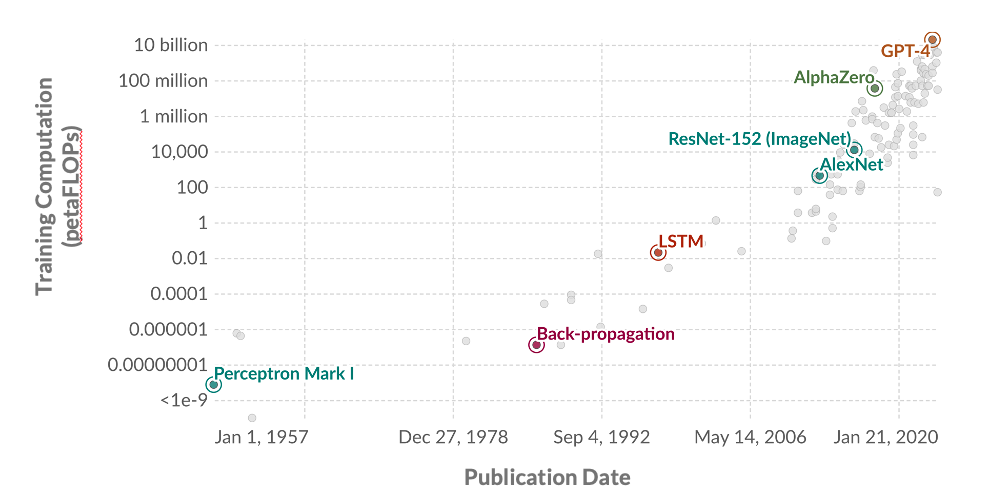
\includegraphics[width=0.7\textwidth]{intro/figures/MLCompute.png}
    \caption{The compute demand of ML models over time. TODO - Make nicer \fillme{}}
    \label{fig:compute_demand}
\end{figure}

% ML has large demand
On the other hand, the supply of compute is struggling to keep up with the demand. Moore's law, which postulates that the number of transistors on a chip doubles every two years, is hitting a wall. As transistors become smaller, reaching the size of a few nanometers, physical limitations such as quantum effects and heat dissipation become significant challenges. This makes it increasingly difficult to continue shrinking components at the pace predicted by Moore's Law. Worse yet, Dennard scaling, which refers to the shrinking of transistors while maintaining constant power density, has ended because of increased leakage currents and heat dissipation issues at smaller transistor sizes. Combined, these factors have led to a plateau in the growth of compute performance.

The growing compute needs of Machine Learning and the shrinking supply of compute for these models has created a supply-demand gap. This gap manifests in two forms - lack of resource availability and high costs of training ML models. \romil{AddMore - Availability - use the news article links, Cost - quote from epochai study} 

% Bridging the gap by making ML more efficient - why we do so.
In this thesis, we bridge the compute supply-demand gap by developing techniques to make machine learning more resource efficient. By optimizing resource utilization, we aim to reduce the overall demand for computational power, thereby easing the pressure on the strained resource supply.

% Looking at the ML stack
How do we improve resource efficiency? Examining the ML stack reveals opportunities across its three layers (Figure \ref{fig:ml_stack}):

\begin{figure}
    \centering
    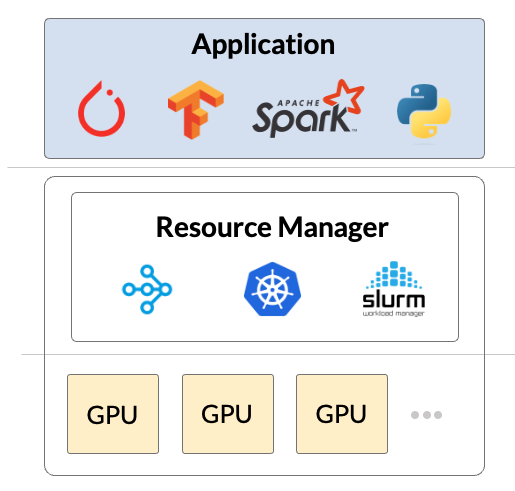
\includegraphics[width=0.5\textwidth]{intro/figures/MLStack.png}
    \caption{The machine learning stack spanning across application, cluster manager, and accelerator layers. TODO - Make nicer \fillme{}}
    \label{fig:ml_stack}
\end{figure}

\begin{enumerate}
\item \textbf{Application Layer:} This layer comprises ML models and their training algorithms. Tools like PyTorch and TensorFlow are commonly used for model definition and workflow specification.
\romil{Orchestration Layer}

\item \textbf{Cluster Manager:} Responsible for managing machine clusters for ML training, this layer oversees job scheduling, resource allocation, and progress tracking, with systems like Kubernetes and Mesos. \romil{ Cluster scheduling/RM layer.}

\item \textbf{Specialized Accelerators:} This hardware layer, including GPUs and TPUs, accelerates ML training, managed by lower-level schedulers. \romil{ML Application Layer - optimizes for inference}
\end{enumerate}

% Ekya - Specialized accelerators
In the accelerator layer, we introduce \textit{Ekya} (Chapter \fillme{}), enhancing the efficiency of continuous learning for high-accuracy inference by 4x. Enabled by the Thief Scheduling algorithm, Ekya innovatively reallocates resources among jobs, focusing on configurations that maximize accuracy improvements for resource costs. The Microprofiler complements this by accurately assessing resource demands and potential accuracy gains, allowing for informed and efficient scheduling decisions. This approach effectively manages resource constraints and addresses data drift challenges.

% Cilantro - Cluster manager
At the cluster manager layer, \textbf{Cilantro} (Chapter \fillme{}) revolutionizes resource allocation by replacing inefficient human-estimated requests with an online learning mechanism. This model forms feedback loops with jobs, creating dynamic resource-to-performance mappings. Cilantro's uncertainty-aware policies, demonstrated in diverse settings, mark a paradigm shift towards more flexible, accurate, and efficient resource allocation.

% Escher - Application layer
Lastly, at the application layer, \textbf{ESCHER} (Chapter \fillme{}) addresses the need for scheduling flexibility without complicating the underlying cluster manager. It introduces ephemeral resources, allowing applications to specify custom scheduling constraints easily. Implemented in Kubernetes and Ray, ESCHER demonstrates enhanced policy expression capabilities, balancing ease-of-use with customizability.

% Conclusion
In conclusion, this thesis presents a comprehensive approach to addressing the compute supply-demand gap in ML. By innovating across the ML stack, it contributes significantly to more efficient resource utilization, paving the way for sustainable and cost-effective ML practices in the face of ever-growing computational demands.

% End of Introduction
\romil{Consider summarizing key contributions and previewing chapters}

